\section*{Question 3}
% \section*{Question 3: Source of Error (Part 2)}

\subsection*{(a)}
% \subsection*{(a) Plot of the Class-Conditional Distributions}
\[
    p(X \mid Y = 1) = \mathrm{Uniform}[1,4], \quad
    p(X \mid Y = 0) = \mathrm{Uniform}[-4,-1].
\]
Thus,
\[
    p(X \mid Y = 1) =
    \begin{cases}
        \frac{1}{3}, & 1 \le X \le 4,    \\
        0,           & \text{otherwise,}
    \end{cases}
    \qquad
    p(X \mid Y = 0) =
    \begin{cases}
        \frac{1}{3}, & -4 \le X \le -1,  \\
        0,           & \text{otherwise.}
    \end{cases}
\]

\begin{figure}[H]
    \centering
    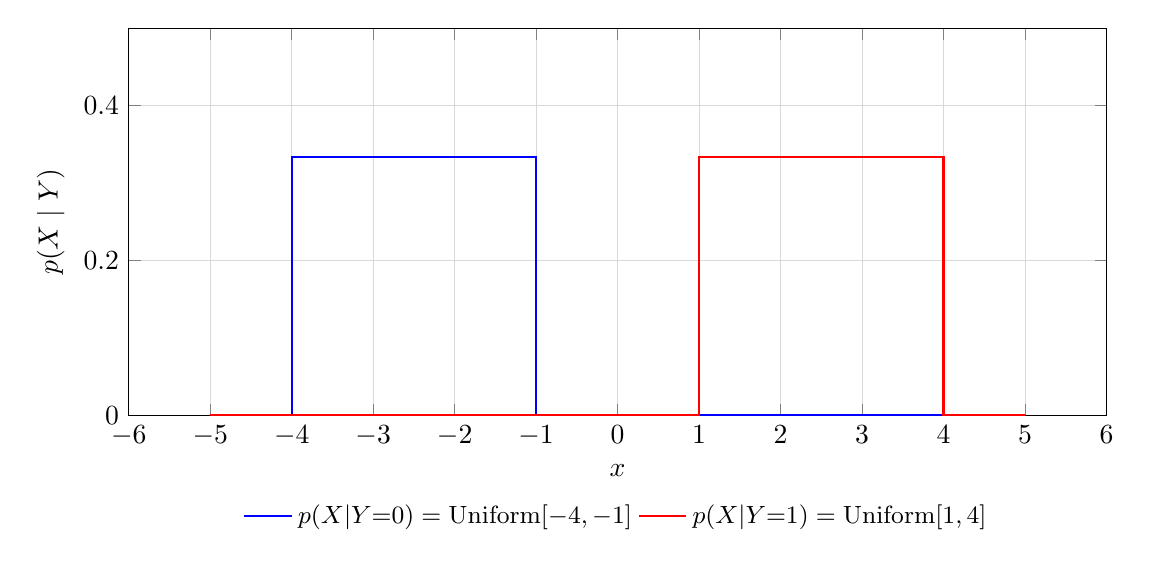
\begin{tikzpicture}
        \begin{axis}[
                width=14cm,
                height=6.5cm,
                xlabel={$x$},
                ylabel={$p(X \mid Y)$},
                ymin=0, ymax=0.5, % 留足空间
                grid=both,
                major grid style={line width=.2pt,draw=gray!30},
                % title={(a) True Class-Conditional Distributions},
                legend style={font=\small, draw=none, fill=none, at={(0.5,-0.2)}, anchor=north, legend columns=2}
            ]
            % 使用 const plot 画均匀分布的“平顶”
            \addplot+[const plot, thick, blue, mark=none] coordinates {(-5,0) (-4,1/3) (-1,1/3) ( -1,0) (5,0)};
            \addlegendentry{$p(X|Y{=}0)=\mathrm{Uniform}[-4,-1]$}

            \addplot+[const plot, thick, red, mark=none] coordinates {(-5,0) (1,1/3) (4,1/3) ( 4,0) (5,0)};
            \addlegendentry{$p(X|Y{=}1)=\mathrm{Uniform}[1,4]$}

        \end{axis}
    \end{tikzpicture}
    % \caption{Non-overlapping uniform class-conditional densities.}
\end{figure}

\subsection*{(b)}
% \subsection*{(b) Error of the Optimal (Bayes) Classifier}
Since the two distributions have disjoint supports and equal priors
\[
    P(Y = 0) = P(Y = 1) = \tfrac{1}{2},
\]
the Bayes classifier simply predicts the class whose support contains $x$. Therefore, the classifier makes no mistakes:
\[
    \boxed{\text{Bayes error} = 0.}
\]

\subsection*{(c)}
% \subsection*{(c) Unavoidable Error for the Modified Case}
% Now consider
\[
    p(X \mid Y = 1) = \mathrm{Uniform}[0,4], \quad
    p(X \mid Y = 0) = \mathrm{Uniform}[-3,1].
\]
% The overlap region is $[0,1]$. Both densities equal $1/4$ in their support regions.
% With equal priors, the Bayes error rate is:
\[
    \text{BayesErr} = \frac{1}{2} \int \min \{ p(x \mid Y=1),\, p(x \mid Y=0) \}\, dx
    = \frac{1}{2} \times \frac{1}{4} \times 1 = \boxed{\tfrac{1}{8} = 0.125.}
\]

\begin{figure}[H]
    \centering
    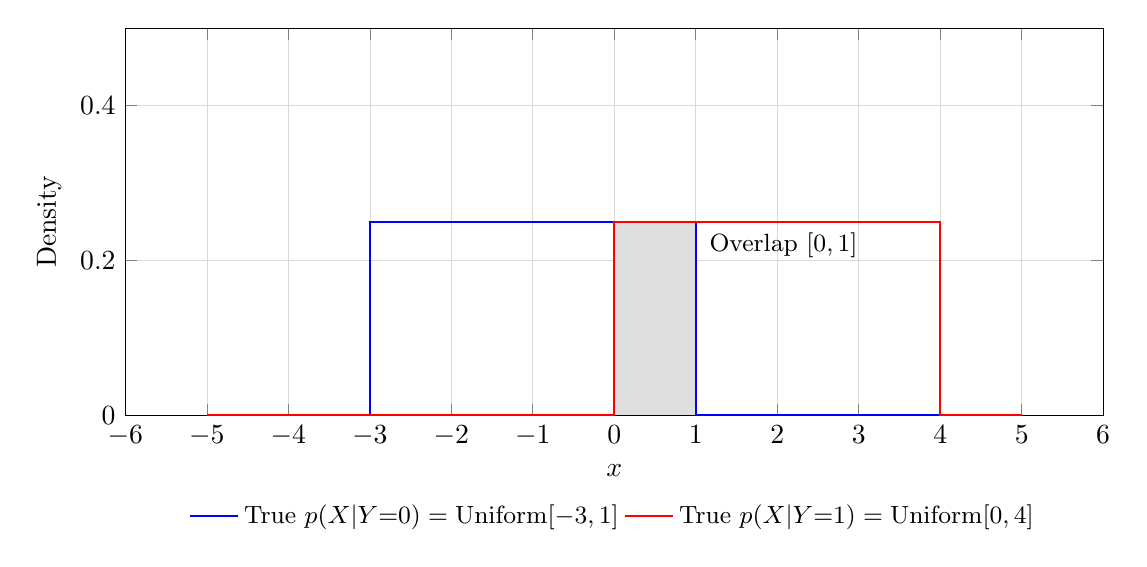
\begin{tikzpicture}
        \begin{axis}[
                width=14cm,
                height=6.5cm,
                xlabel={$x$},
                ylabel={Density},
                ymin=0, ymax=0.5,
                grid=both,
                major grid style={line width=.2pt,draw=gray!30},
                % title={(c) Overlapping Uniforms and Unavoidable Error},
                legend style={font=\small, draw=none, fill=none, at={(0.5,-0.2)}, anchor=north, legend columns=2}
            ]
            % 阴影:overlap [0,1],高度=1/4
            \path [fill=gray!25] (axis cs:0,0) rectangle (axis cs:1,0.25);

            % p(X|Y=0) = Uniform[-3,1]
            \addplot+[const plot, thick, blue, mark=none] coordinates {(-5,0) (-3,0.25) (1,0.25) (1,0) (5,0)};
            \addlegendentry{True $p(X|Y{=}0)=\mathrm{Uniform}[-3,1]$}

            % p(X|Y=1) = Uniform[0,4]
            \addplot+[const plot, thick, red, mark=none] coordinates {(-5,0) (0,0.25) (4,0.25) (4,0) (5,0)};
            \addlegendentry{True $p(X|Y{=}1)=\mathrm{Uniform}[0,4]$}

            \node[anchor=west] at (axis cs:1.05,0.22) {\small Overlap $[0,1]$};

        \end{axis}
    \end{tikzpicture}
    % \caption{Overlap region $[0,1]$ (shaded) yields Bayes error $\frac{1}{2}\cdot\frac{1}{4}\cdot 1=\frac{1}{8}$.}
\end{figure}


\subsection*{(d)}
% \subsection*{(d) Gaussian Naive Bayes (GNB) with Infinite Data}
% Under the setting of part (a), a Gaussian Naive Bayes model incorrectly assumes that
% each class-conditional distribution is Gaussian.
For a uniform distribution $\mathrm{Uniform}[a,b]$, we have:
\[
    \mu = \frac{a+b}{2}, \qquad \sigma^2 = \frac{(b-a)^2}{12}.
\]
Hence,
\[
    p(X \mid Y=0) \approx \mathcal{N}(-2.5,\, 0.75), \qquad
    p(X \mid Y=1) \approx \mathcal{N}(2.5,\, 0.75).
\]
With equal priors and identical variances, the decision boundary occurs at:
\[
    x^* = \frac{\mu_0 + \mu_1}{2} = 0.
\]
Therefore, the classifier predicts $Y=1$ if $x>0$, and $Y=0$ otherwise.

The classification error of GNB is:
\[
    \mathrm{Err}_{\mathrm{GNB}}
    = \frac{1}{2} \int_{-4}^{-1} \mathbf{1}\{x > x^*\}\,\frac{1}{3}\, dx
    + \frac{1}{2} \int_{1}^{4} \mathbf{1}\{x < x^*\}\,\frac{1}{3}\, dx.
\]
Since the threshold $x^*=0$ lies between the two non-overlapping intervals,
both integrals are zero and thus:
\[
    \boxed{\mathrm{Err}_{\mathrm{GNB}} = 0.}
\]
Although the GNB model is biased (it cannot represent the true uniform shape),
the symmetry of the problem yields zero misclassification error.

\begin{figure}[H]
    \centering
    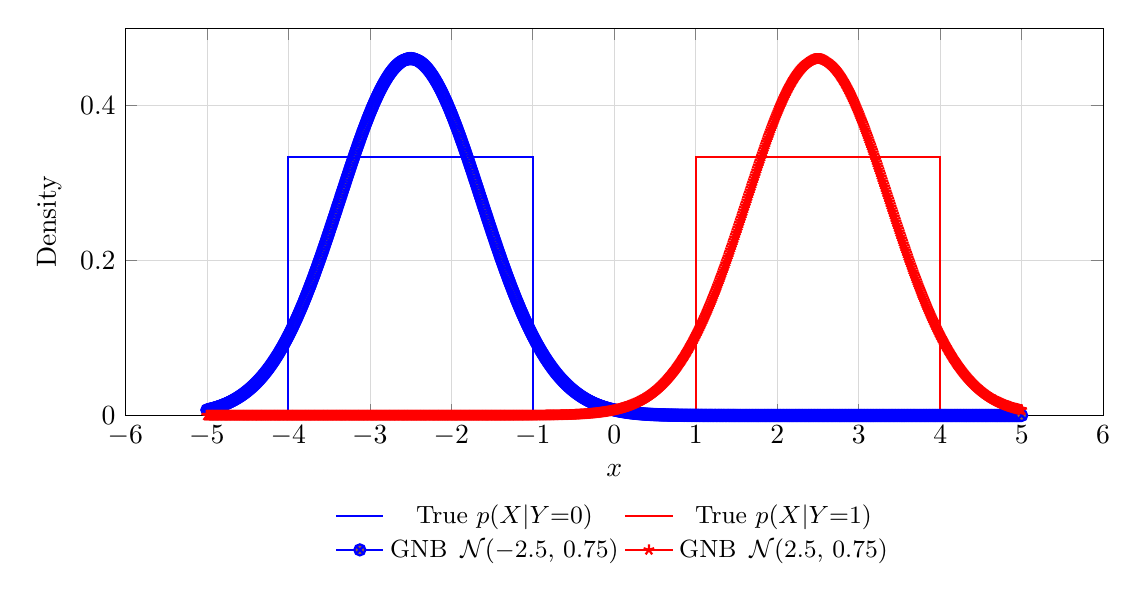
\begin{tikzpicture}
        \begin{axis}[
                width=14cm,
                height=6.5cm,
                xlabel={$x$},
                ylabel={Density},
                ymin=0, ymax=0.5, % 0.46 的峰值不会被截断
                grid=both,
                major grid style={line width=.2pt,draw=gray!30},
                % title={(d) True vs.\ GNB-Fitted Class-Conditional Densities},
                legend style={font=\small, draw=none, fill=none, at={(0.5,-0.2)}, anchor=north, legend columns=2}
            ]
            % True uniforms with const plot
            \addplot+[const plot, thick, blue, mark=none] coordinates {(-5,0) (-4,1/3) (-1,1/3) (-1,0) (5,0)};
            \addlegendentry{True $p(X|Y{=}0)$}

            \addplot+[const plot, thick, red, mark=none] coordinates {(-5,0) (1,1/3) (4,1/3) (4,0) (5,0)};
            \addlegendentry{True $p(X|Y{=}1)$}

            % GNB Gaussian fits (samples up)
            \addplot+[domain=-5:5, samples=1000, thick, blue]
            {1/sqrt(2*pi*0.75)*exp(-((x+2.5)^2)/(2*0.75))};
            \addlegendentry{GNB $\,\mathcal{N}(-2.5,\,0.75)$}

            \addplot+[domain=-5:5, samples=1000, thick, red]
            {1/sqrt(2*pi*0.75)*exp(-((x-2.5)^2)/(2*0.75))};
            \addlegendentry{GNB $\,\mathcal{N}(2.5,\,0.75)$}

        \end{axis}
    \end{tikzpicture}
    % \caption{Uniform ground-truth vs.\ Gaussian Naive Bayes fits ($n\!\to\!\infty$).}
\end{figure}



\subsection*{(e)}
% \subsection*{(e) Effect of Finite Training Data}

With a finite $n$, the estimated class means and variances,
$\hat\mu_k,\hat\sigma_k^2$, fluctuate due to sampling noise.

Consequently, the GNB decision rule (and its threshold) fluctuates as well.

This introduces a \boxed{\emph{variance}} component of error on top of the (model) \emph{bias}.